%!TEX root=../main.tex
\section{On the geometry of multivariate functional data} % (fold)
\label{sec:geometric_point_of_view_mfpca}

\subsection{Duality diagram} % (fold)
\label{sub:duality_diagram}

\textcolor{red}{Check if it's OK with the centering.}

\add{The distinction between the space of rows of a matrix as a sample from a population and the space of columns as the fixed variables on which the observations were measured has been explained in \cite{holmesMultivariateDataAnalysis2008,delacruzDualityDiagramData2011} for multivariate data analysis. We propose to define a duality diagram in the context of multivariate functional data. Consider the data matrix defined by the set $\mathcal{X}$. We define an operator $L_X : \HH \rightarrow \RR^N$ by
\begin{equation}
    L_X: u \mapsto \begin{pmatrix}
        \inH{X_1 - \mu}{u} \\
        \vdots \\
        \inH{X_N - \mu}{u}
    \end{pmatrix}.
\end{equation}
Using the linearity of the inner-product $\inH{\cdot}{\cdot}$ and vectors, the operator $L_X$ is linear. The adjoint operator of $L_X$ is given by
\begin{equation}
    L^\star_X: v \mapsto \begin{pmatrix}
       \sum_{n = 1}^N v_n \{X_n^{(1)}(t_1) - \mup{1}(t_1)\} \\ 
       \vdots \\ 
       \sum_{n = 1}^N v_n \{X_n^{(P)}(t_P) - \mup{P}(t_P)\}
    \end{pmatrix}.
\end{equation}
As $L^\star_X$ is the adjoint of the linear operator $L_X$, it is a linear operator. 
We consider the function $\inHG{f}{g} = \inH{f}{\Gamma g}, f, g \in \HH$ and $\inRM{u}{v} = u^\top M v, u, v \in \RR^N$.
These relationship can be expressed as a duality diagram, see Figure~\ref{fig:duality_diagram}. The triplet $(X, \Gamma, M)$ defines a (multivariate) functional data analysis setup. The estimation of the eigencomponents can be performed using $\Gamma$ or $M$ and the relationship between the two are derived in Section~\ref{sec:functional_principal_components_analysis}.}
\begin{figure}
    \centering
    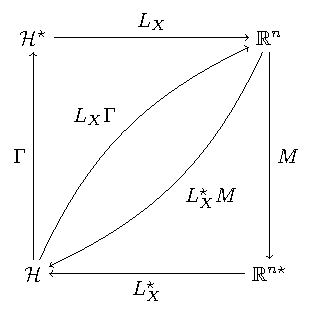
\includegraphics[scale=1.2]{figures/duality_diagram.pdf}
    \caption{Duality diagram between the spaces $\mathcal{H}$ and $\mathbb{R}^N$. The operator $L_X$ and its adjoint $L^\star_X$ are linear operators. The covariance operator $\Gamma$ and the matrix $M$ define geometries in $\mathcal{H}$ and $\mathbb{R}^N$ respectively. The space $\HH^\star$ (resp. $\RR^{N \star}$) is the dual space of $\HH$ (resp. $\RR^N$).}
    \label{fig:duality_diagram}
\end{figure}


% subsection duality_diagram (end)

\subsection{Cloud of individuals} % (fold)
\label{sub:cloud_of_individuals}

Given $n \in \{1, \dots, N\}$, let $\{\Xnp(t_p),\,t_p \in \TT{p},\,p = 1, \dots, P\}$ be the features set for a particular observation $n$. We identify this set as the point $\pobs{M}_n$ in the space $\HH$. The space $\HH$ is referred to as the observations' space. The cloud of points that represents the set of observations in $\HH$ is denoted by $\CN$. Let $\GN$ be the centre of gravity of the cloud $\CN$. In the space $\HH$, its coordinates are given by $\{\mup{p}(t_p),\,t_p \in \TT{p},\,p = 1, \dots, P\}$. If the features are centered, the origin $\OH$ of the axes in $\HH$ coincides with $\GN$.

\begin{figure}
    \centering
    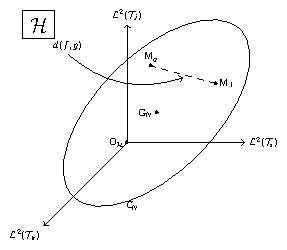
\includegraphics[scale=1.2]{figures/cloud_obs.pdf}
    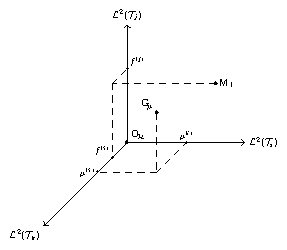
\includegraphics[scale=1.2]{figures/cloud_obs_proj.pdf}
    \caption{\add{Left: Cloud of observations. Right: Projection of the points onto the elements of $\HH$. The observation $f$ (resp. $g$) is identified by the point $\pobs{M}_f$ (resp. $\pobs{M}_g$) in the cloud $\CN$. The point $\GN$ is the center of gravity of $\CN$ and the point $\OH$ is the origin of the space $\HH$.}}
    \label{fig:cloud_obs}
\end{figure}

Let $f$ and $g$ be two elements in $\HH$ and denote by $\pobs{M}_f$ and $\pobs{M}_g$ their associated points in $\CN$ (see Figure~\ref{fig:cloud_obs}). The distance between these observations is defined as
\begin{equation}\label{eq:distance_obs}
    d^2(\pobs{M}_f, \pobs{M}_g) = \normH{f - g}^2 = \sum_{p = 1}^P \int_{\TT{p}}\left\{\fp(t_p) - \gp(t_p)\right\}^2 \dd t_p.
\end{equation}
This distance measures how different the observations are, and thus characterizes the shape of the cloud $\CN$. Another description of this shape is to consider the distance between each observation and $\GN$, the center of the cloud. Let $f$ be an element of $\HH$, associated to the point $\pobs{M}_f$, and $\mu$ the element of $\HH$ related to $\GN$, the distance between $f$ and $\mu$ is given by
\begin{equation}\label{eq:distance_center}
    d^2(\pobs{M}_f, \GN) = \normH{f - \mu}^2 = \sum_{p = 1}^P \int_{\TT{p}}\left\{\fp(t_p) - \mup{p}(t_p)\right\}^2 \dd t_p.
\end{equation}
Given the set $\XX$, the total inertia of $\CN$, with respect to $\GN$, is given by
\begin{equation}\label{eq:inertia}
    \sum_{n = 1}^N \pi_n d^2(\pobs{M}_n, \GN) = \frac{1}{2}\sum_{i = 1}^N \sum_{j = 1}^N \pi_i \pi_j d^2(\pobs{M}_i, \pobs{M}_j) = \sum_{p = 1}^P \int_{\TT{p}}\Var{\Xp{p}(t_p)} \dd t_p.
\end{equation}
The derivation of these equalities are given in Appendix \ref{sec:derivation_of_the_inertia_of_the_clouds}.

\begin{remark}
    These results have the same interpretation as for multivariate scalar data. This is also the multivariate analogue of the relation between variance and sum of squared differences known for univariate functional data. If the features are reduced beforehand, the total inertia of the cloud $\CN$ is equal to the number of components $P$. We are, in general, not interested by the total inertia but mostly how this variance is spread among the features.
\end{remark}

% subsection cloud_of_individuals (end)

\subsection{Cloud of features} % (fold)
\label{sub:cloud_of_features}

\add{Given an element $f \in \HH$, let $\{\inH{X_n - \mu}{f}, n = 1, \dots, N\}$ be the set of projections of $f$ on the observations. We identify this set as the point $\pfea{M}_f$ in the space $\RR^N$. The space $\RR^N$ is referred to as the features' space. The cloud of points that represents the set of observations in $\RR^N$ is denoted by $\CP$. The origin $\OG$ of the axes in $\RR^N$ coincides with the centre of gravity of the cloud $\CP$. We consider the usual inner-product in $\RR^N$. Let $f$ and $g$ be two elements in $\HH$ and denote by $\pfea{M}_f$ and $\pfea{M}_g$ their associated points in $\CP$ (see Figure~\ref{fig:cloud_features}). The distance between $\pfea{M}_f$ and $\pfea{M}_g$ is thus defined as
\begin{equation*}
d^2(\pfea{M}_f, \pfea{M}_g) = \sum_{n = 1}^N \pi_n \inH{X_n - \mu}{f - g}.
\end{equation*}
Let $f$ be an element of $\HH$, associated to the point $\pfea{M}_f$, the distance between $\pfea{M}_f$ and $\OG$ is given by
\begin{equation*}
d^2(\pfea{M}_f, \OG) = \sum_{n = 1}^N \pi_n \inH{X_n - \mu}{f}.
\end{equation*}
\begin{equation}
    \cos(\theta_{fg}) = \frac{\sum_{n = 1}^N \pi_n \inH{X_n - \mu}{f}\inH{X_n - \mu}{g}}{\left(\sum_{n = 1}^N \pi_n \inH{X_n - \mu}{f}^2\right)^{1/2}\left(\sum_{n = 1}^N \pi_n \inH{X_n - \mu}{g}^2\right)^{1/2}}.
\end{equation}
}

\begin{figure}
    \centering
    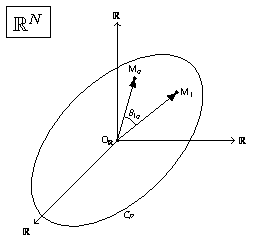
\includegraphics[scale=1.2]{figures/cloud_features.pdf}
    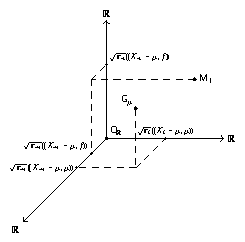
\includegraphics[scale=1.2]{figures/cloud_features_proj.pdf}
    \caption{\add{Left: Cloud of features. Right: Projection of the points on the elements of $\RR^N$. The observation $f$ (resp. $g$) is identified by the point $\pfea{M}_f$ (resp. $\pfea{M}_g$) in the cloud $\CP$. The point $\OG$ is the origin of the space $\RR^N$ (and coincide with the center of gravity of $\CP$).}}
    \label{fig:cloud_features}
\end{figure}

\begin{remark}
   \add{Although each axis of the space does not directly represent the features, but rather the projection of an element of $\HH$ onto the elements of the set $\XX$, we refer to this space as the features' space. We use this terminology to highlight the similarity between multivariate functional data analysis and traditional multivariate data analysis, as well as to emphasize the dimensionality of this space.}
\end{remark}
% subsection cloud_of_features (end)

\subsection{On centering and reducing} % (fold)
\label{sub:on_centering_and_reducing}

For conducting an MFPCA, the features are usually assumed centred \citep{happMultivariateFunctionalPrincipal2018a}. \cite{protheroNewPerspectivesCentering2021} give a complete overview of centering in the context of FDA. Here, we comment on the geometric interpretation of centering in this context and compare with the multivariate scalar case. We focus on the usual centering in FDA, namely $\Xnp(t_p) - \mu^{(p)}(t_p),~t_p \in \TT{p}$ (refered as \emph{object centering} in \cite{protheroNewPerspectivesCentering2021}).
The geometric interpretation of the centering differs if we refer to the observations' space $\HH$ or the features' space $\RR^N$. Within the space $\HH$, centering is interpreted as translating the centre of gravity of the curves $\GN$ to the origin point $\OH$ of $\HH$. This transformation, being a translation, does not change the shape of the cloud $\CN$. The interpretation is the same as for the multivariate scalar data. Within the space $\RR^N$, the centering is harder to interpret and does not have the same meaning as in the multivariate case. Actually, in the multivariate scalar case, the centering of the data can be geometrically interpreted as the projection of the data on the subspace orthogonal to the constant vector. However, what happens if we project the multivariate curves onto the vector (of length $P$) of constant functions?

\add{In the features' space, the inner product is the usual Euclidean inner-product.
\begin{equation}
\inH{f}{g} = \sum_{i = 1}^N \int_{\TT{k}} f^{(k)}_i(t)g^{(k)}_i(t)dt, \quad f, g \in \GG.
\end{equation}
Let $\mathbf{1}$ be the vector of constant function in $\GG$ and $f$ an element of $\GG$. The projection of $f$ onto $\mathbf{1}$ is then given by
\begin{equation}
P_{\mathbf{1}}f = \frac{\inH{f}{\mathbf{1}}}{\normH{\mathbf{1}}}\mathbf{1} = \frac{1}{N\lvert \TT{k} \rvert}\sum_{n = 1}^N \int_{\TT{k}} f^{(k)}_n(t)dt\mathbf{1}
\end{equation}
In practice, this is equivalent to computing the mean value of the mean curve for each component, referred as \emph{grand mean centering} in \cite{protheroNewPerspectivesCentering2021}.}

Concerning the standardization of the data, there are mainly two proposal in the literature. \cite{happMultivariateFunctionalPrincipal2018a} propose to weight each component $p$ by
\begin{equation}
w_p = \left(\int_{\TT{p}} \Var X^{(p)}(t_p) \dd t_p\right)^{-1}.
\end{equation}
This standardization is coherent with the derivation of the total inertia of the observations' space. Using these weights, the total inertia of $\CN$ is equal to the number of components $P$. \cite{chiouMultivariateFunctionalPrincipal2014} propose to standardize each component $p$ of the data using the function
\begin{equation}
w_p(t_p) = \left(\Var X^{(p)}(t_p)\right)^{-1/2}, \quad t_p \in \TT{p}.
\end{equation}
This corresponds to a standardization of the curves by the standard deviation of the component at each sampling point. The standard deviation curve is estimated as the square root of the diagonal of the covariance function estimates, obtained using a local linear smoother of the pooled data. 

% subsection on_centering_and_reducing (end)

% section sec:geometric_point_of_view_mfpca (end)